\documentclass[1p]{elsarticle_modified}
%\bibliographystyle{elsarticle-num}

%\usepackage[colorlinks]{hyperref}
%\usepackage{abbrmath_seonhwa} %\Abb, \Ascr, \Acal ,\Abf, \Afrak
\usepackage{amsfonts}
\usepackage{amssymb}
\usepackage{amsmath}
\usepackage{amsthm}
\usepackage{scalefnt}
\usepackage{amsbsy}
\usepackage{kotex}
\usepackage{caption}
\usepackage{subfig}
\usepackage{color}
\usepackage{graphicx}
\usepackage{xcolor} %% white, black, red, green, blue, cyan, magenta, yellow
\usepackage{float}
\usepackage{setspace}
\usepackage{hyperref}

\usepackage{tikz}
\usetikzlibrary{arrows}

\usepackage{multirow}
\usepackage{array} % fixed length table
\usepackage{hhline}

%%%%%%%%%%%%%%%%%%%%%
\makeatletter
\renewcommand*\env@matrix[1][\arraystretch]{%
	\edef\arraystretch{#1}%
	\hskip -\arraycolsep
	\let\@ifnextchar\new@ifnextchar
	\array{*\c@MaxMatrixCols c}}
\makeatother %https://tex.stackexchange.com/questions/14071/how-can-i-increase-the-line-spacing-in-a-matrix
%%%%%%%%%%%%%%%

\usepackage[normalem]{ulem}

\newcommand{\msout}[1]{\ifmmode\text{\sout{\ensuremath{#1}}}\else\sout{#1}\fi}
%SOURCE: \msout is \stkout macro in https://tex.stackexchange.com/questions/20609/strikeout-in-math-mode

\newcommand{\cancel}[1]{
	\ifmmode
	{\color{red}\msout{#1}}
	\else
	{\color{red}\sout{#1}}
	\fi
}

\newcommand{\add}[1]{
	{\color{blue}\uwave{#1}}
}

\newcommand{\replace}[2]{
	\ifmmode
	{\color{red}\msout{#1}}{\color{blue}\uwave{#2}}
	\else
	{\color{red}\sout{#1}}{\color{blue}\uwave{#2}}
	\fi
}

\newcommand{\Sol}{\mathcal{S}} %segment
\newcommand{\D}{D} %diagram
\newcommand{\A}{\mathcal{A}} %arc


%%%%%%%%%%%%%%%%%%%%%%%%%%%%%5 test

\def\sl{\operatorname{\textup{SL}}(2,\Cbb)}
\def\psl{\operatorname{\textup{PSL}}(2,\Cbb)}
\def\quan{\mkern 1mu \triangleright \mkern 1mu}

\theoremstyle{definition}
\newtheorem{thm}{Theorem}[section]
\newtheorem{prop}[thm]{Proposition}
\newtheorem{lem}[thm]{Lemma}
\newtheorem{ques}[thm]{Question}
\newtheorem{cor}[thm]{Corollary}
\newtheorem{defn}[thm]{Definition}
\newtheorem{exam}[thm]{Example}
\newtheorem{rmk}[thm]{Remark}
\newtheorem{alg}[thm]{Algorithm}

\newcommand{\I}{\sqrt{-1}}
\begin{document}

%\begin{frontmatter}
%
%\title{Boundary parabolic representations of knots up to 8 crossings}
%
%%% Group authors per affiliation:
%\author{Yunhi Cho} 
%\address{Department of Mathematics, University of Seoul, Seoul, Korea}
%\ead{yhcho@uos.ac.kr}
%
%
%\author{Seonhwa Kim} %\fnref{s_kim}}
%\address{Center for Geometry and Physics, Institute for Basic Science, Pohang, 37673, Korea}
%\ead{ryeona17@ibs.re.kr}
%
%\author{Hyuk Kim}
%\address{Department of Mathematical Sciences, Seoul National University, Seoul 08826, Korea}
%\ead{hyukkim@snu.ac.kr}
%
%\author{Seokbeom Yoon}
%\address{Department of Mathematical Sciences, Seoul National University, Seoul, 08826,  Korea}
%\ead{sbyoon15@snu.ac.kr}
%
%\begin{abstract}
%We find all boundary parabolic representation of knots up to 8 crossings.
%
%\end{abstract}
%\begin{keyword}
%    \MSC[2010] 57M25 
%\end{keyword}
%
%\end{frontmatter}

%\linenumbers
%\tableofcontents
%
\newcommand\colored[1]{\textcolor{white}{\rule[-0.35ex]{0.8em}{1.4ex}}\kern-0.8em\color{red} #1}%
%\newcommand\colored[1]{\textcolor{white}{ #1}\kern-2.17ex	\textcolor{white}{ #1}\kern-1.81ex	\textcolor{white}{ #1}\kern-2.15ex\color{red}#1	}

{\Large $\underline{12a_{0102}~(K12a_{0102})}$}

\setlength{\tabcolsep}{10pt}
\renewcommand{\arraystretch}{1.6}
\vspace{1cm}\begin{tabular}{m{100pt}>{\centering\arraybackslash}m{274pt}}
\multirow{5}{120pt}{
	\centering
	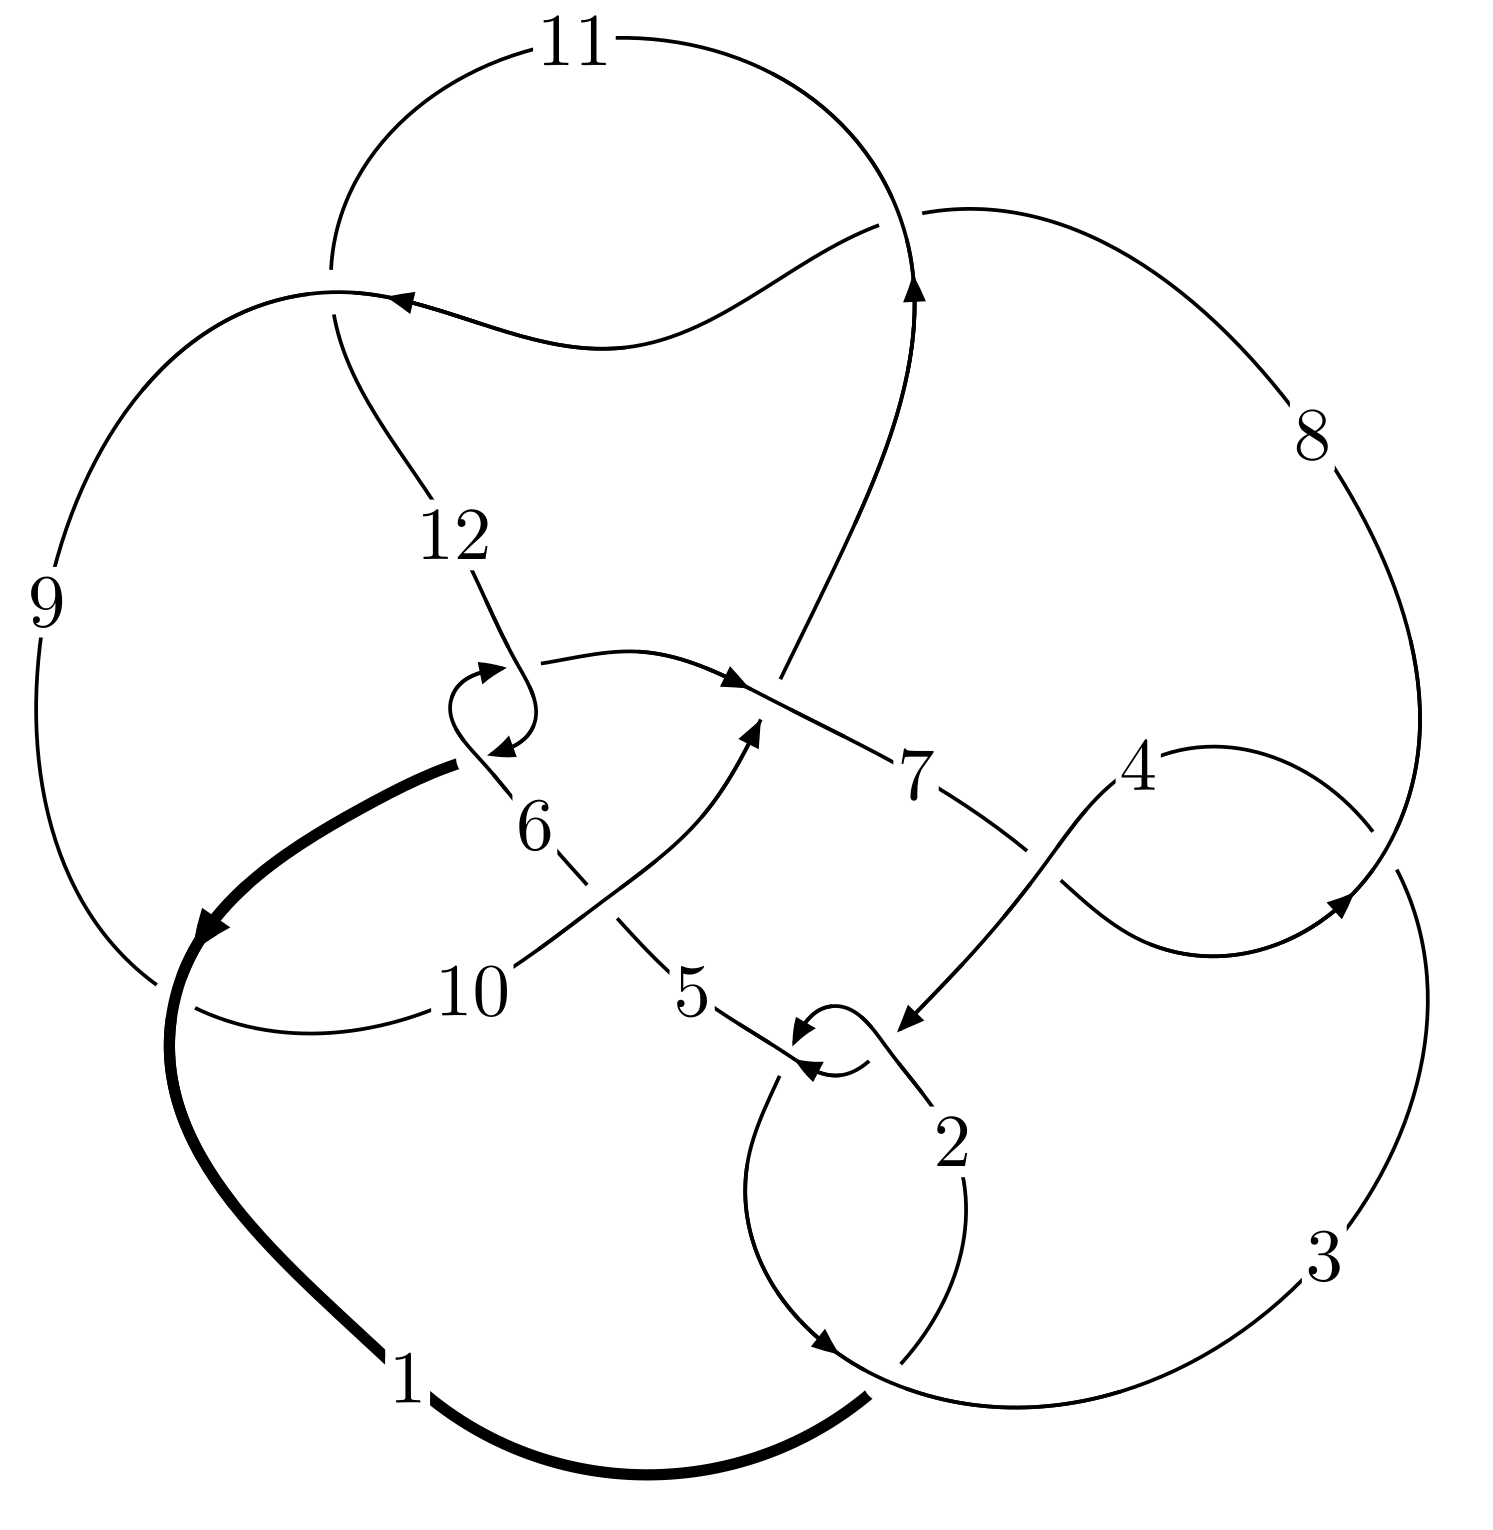
\includegraphics[width=112pt]{../../../GIT/diagram.site/Diagrams/png/903_12a_0102.png}\\
\ \ \ A knot diagram\footnotemark}&
\allowdisplaybreaks
\textbf{Linearized knot diagam} \\
\cline{2-2}
 &
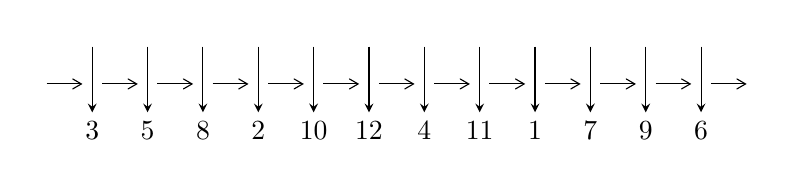
\begin{tikzpicture}[x=20pt, y=17pt]
	% nodes
	\node (C0) at (0, 0) {};
	\node (C1) at (1, 0) {};
	\node (C1U) at (1, +1) {};
	\node (C1D) at (1, -1) {3};

	\node (C2) at (2, 0) {};
	\node (C2U) at (2, +1) {};
	\node (C2D) at (2, -1) {5};

	\node (C3) at (3, 0) {};
	\node (C3U) at (3, +1) {};
	\node (C3D) at (3, -1) {8};

	\node (C4) at (4, 0) {};
	\node (C4U) at (4, +1) {};
	\node (C4D) at (4, -1) {2};

	\node (C5) at (5, 0) {};
	\node (C5U) at (5, +1) {};
	\node (C5D) at (5, -1) {10};

	\node (C6) at (6, 0) {};
	\node (C6U) at (6, +1) {};
	\node (C6D) at (6, -1) {12};

	\node (C7) at (7, 0) {};
	\node (C7U) at (7, +1) {};
	\node (C7D) at (7, -1) {4};

	\node (C8) at (8, 0) {};
	\node (C8U) at (8, +1) {};
	\node (C8D) at (8, -1) {11};

	\node (C9) at (9, 0) {};
	\node (C9U) at (9, +1) {};
	\node (C9D) at (9, -1) {1};

	\node (C10) at (10, 0) {};
	\node (C10U) at (10, +1) {};
	\node (C10D) at (10, -1) {7};

	\node (C11) at (11, 0) {};
	\node (C11U) at (11, +1) {};
	\node (C11D) at (11, -1) {9};

	\node (C12) at (12, 0) {};
	\node (C12U) at (12, +1) {};
	\node (C12D) at (12, -1) {6};
	\node (C13) at (13, 0) {};

	% arrows
	\draw[->,>={angle 60}]
	(C0) edge (C1) (C1) edge (C2) (C2) edge (C3) (C3) edge (C4) (C4) edge (C5) (C5) edge (C6) (C6) edge (C7) (C7) edge (C8) (C8) edge (C9) (C9) edge (C10) (C10) edge (C11) (C11) edge (C12) (C12) edge (C13) ;	\draw[->,>=stealth]
	(C1U) edge (C1D) (C2U) edge (C2D) (C3U) edge (C3D) (C4U) edge (C4D) (C5U) edge (C5D) (C6U) edge (C6D) (C7U) edge (C7D) (C8U) edge (C8D) (C9U) edge (C9D) (C10U) edge (C10D) (C11U) edge (C11D) (C12U) edge (C12D) ;
	\end{tikzpicture} \\
\hhline{~~} \\& 
\textbf{Solving Sequence} \\ \cline{2-2} 
 &
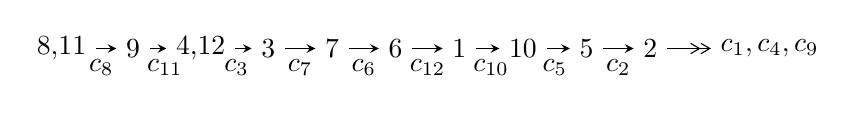
\begin{tikzpicture}[x=23pt, y=7pt]
	% node
	\node (A0) at (-1/8, 0) {8,11};
	\node (A1) at (1, 0) {9};
	\node (A2) at (33/16, 0) {4,12};
	\node (A3) at (25/8, 0) {3};
	\node (A4) at (33/8, 0) {7};
	\node (A5) at (41/8, 0) {6};
	\node (A6) at (49/8, 0) {1};
	\node (A7) at (57/8, 0) {10};
	\node (A8) at (65/8, 0) {5};
	\node (A9) at (73/8, 0) {2};
	\node (C1) at (1/2, -1) {$c_{8}$};
	\node (C2) at (3/2, -1) {$c_{11}$};
	\node (C3) at (21/8, -1) {$c_{3}$};
	\node (C4) at (29/8, -1) {$c_{7}$};
	\node (C5) at (37/8, -1) {$c_{6}$};
	\node (C6) at (45/8, -1) {$c_{12}$};
	\node (C7) at (53/8, -1) {$c_{10}$};
	\node (C8) at (61/8, -1) {$c_{5}$};
	\node (C9) at (69/8, -1) {$c_{2}$};
	\node (A10) at (11, 0) {$c_{1},c_{4},c_{9}$};

	% edge
	\draw[->,>=stealth]	
	(A0) edge (A1) (A1) edge (A2) (A2) edge (A3) (A3) edge (A4) (A4) edge (A5) (A5) edge (A6) (A6) edge (A7) (A7) edge (A8) (A8) edge (A9) ;
	\draw[->>,>={angle 60}]	
	(A9) edge (A10);
\end{tikzpicture} \\ 

\end{tabular} \\

\footnotetext{
The image of knot diagram is generated by the software ``\textbf{Draw programme}" developed by Andrew Bartholomew(\url{http://www.layer8.co.uk/maths/draw/index.htm\#Running-draw}), where we modified some parts for our purpose(\url{https://github.com/CATsTAILs/LinksPainter}).
}\phantom \\ \newline 
\centering \textbf{Ideals for irreducible components\footnotemark of $X_{\text{par}}$} 
 
\begin{align*}
I^u_{1}&=\langle 
-2.86118\times10^{608} u^{128}-9.03918\times10^{608} u^{127}+\cdots+3.04756\times10^{609} b-2.75259\times10^{610},\\
\phantom{I^u_{1}}&\phantom{= \langle  }2.19044\times10^{608} u^{128}+9.28924\times10^{608} u^{127}+\cdots+4.57134\times10^{609} a-5.57993\times10^{610},\\
\phantom{I^u_{1}}&\phantom{= \langle  }u^{129}+4 u^{128}+\cdots+810 u+81\rangle \\
I^u_{2}&=\langle 
b,\;u^7+2 u^6-2 u^5-4 u^4+2 u^3+2 u^2+a+2,\;u^8+u^7-3 u^6-2 u^5+3 u^4+2 u-1\rangle \\
I^u_{3}&=\langle 
2 b-3 a-2,\;9 a^2+6 a-4,\;u-1\rangle \\
\\
\end{align*}
\raggedright * 3 irreducible components of $\dim_{\mathbb{C}}=0$, with total 139 representations.\\
\footnotetext{All coefficients of polynomials are rational numbers. But the coefficients are sometimes approximated in decimal forms when there is not enough margin.}
\newpage
\renewcommand{\arraystretch}{1}
\centering \section*{I. $I^u_{1}= \langle -2.86\times10^{608} u^{128}-9.04\times10^{608} u^{127}+\cdots+3.05\times10^{609} b-2.75\times10^{610},\;2.19\times10^{608} u^{128}+9.29\times10^{608} u^{127}+\cdots+4.57\times10^{609} a-5.58\times10^{610},\;u^{129}+4 u^{128}+\cdots+810 u+81 \rangle$}
\flushleft \textbf{(i) Arc colorings}\\
\begin{tabular}{m{7pt} m{180pt} m{7pt} m{180pt} }
\flushright $a_{8}=$&$\begin{pmatrix}1\\0\end{pmatrix}$ \\
\flushright $a_{11}=$&$\begin{pmatrix}0\\u\end{pmatrix}$ \\
\flushright $a_{9}=$&$\begin{pmatrix}1\\u^2\end{pmatrix}$ \\
\flushright $a_{4}=$&$\begin{pmatrix}-0.0479167 u^{128}-0.203206 u^{127}+\cdots+38.5131 u+12.2063\\0.0938842 u^{128}+0.296604 u^{127}+\cdots+73.2334 u+9.03212\end{pmatrix}$ \\
\flushright $a_{12}=$&$\begin{pmatrix}- u\\- u^3+u\end{pmatrix}$ \\
\flushright $a_{3}=$&$\begin{pmatrix}0.0459675 u^{128}+0.0933979 u^{127}+\cdots+111.746 u+21.2385\\0.0938842 u^{128}+0.296604 u^{127}+\cdots+73.2334 u+9.03212\end{pmatrix}$ \\
\flushright $a_{7}=$&$\begin{pmatrix}-0.0705351 u^{128}-0.229615 u^{127}+\cdots-22.0216 u-8.44795\\-0.174404 u^{128}-0.559025 u^{127}+\cdots-129.629 u-14.8100\end{pmatrix}$ \\
\flushright $a_{6}=$&$\begin{pmatrix}-0.217094 u^{128}-0.708408 u^{127}+\cdots-147.263 u-22.5766\\-0.108675 u^{128}-0.354830 u^{127}+\cdots-79.5453 u-9.38430\end{pmatrix}$ \\
\flushright $a_{1}=$&$\begin{pmatrix}0.0402884 u^{128}+0.0431499 u^{127}+\cdots-3.07411 u-5.90774\\0.0971169 u^{128}+0.306541 u^{127}+\cdots+72.8538 u+7.09885\end{pmatrix}$ \\
\flushright $a_{10}=$&$\begin{pmatrix}0.0935044 u^{128}+0.442842 u^{127}+\cdots+39.1713 u+9.65066\\0.00292730 u^{128}+0.0528804 u^{127}+\cdots-21.8667 u-0.921416\end{pmatrix}$ \\
\flushright $a_{5}=$&$\begin{pmatrix}-0.129678 u^{128}-0.378848 u^{127}+\cdots-146.629 u-20.5705\\-0.0423601 u^{128}-0.133841 u^{127}+\cdots-42.7148 u-5.05621\end{pmatrix}$ \\
\flushright $a_{2}=$&$\begin{pmatrix}-0.124068 u^{128}-0.463817 u^{127}+\cdots-29.7332 u+0.392563\\0.0423601 u^{128}+0.133841 u^{127}+\cdots+42.7148 u+5.05621\end{pmatrix}$\\&\end{tabular}
\flushleft \textbf{(ii) Obstruction class $= -1$}\\~\\
\flushleft \textbf{(iii) Cusp Shapes $= -0.612839 u^{128}-1.98956 u^{127}+\cdots-336.700 u-48.6406$}\\~\\
\newpage\renewcommand{\arraystretch}{1}
\flushleft \textbf{(iv) u-Polynomials at the component}\newline \\
\begin{tabular}{m{50pt}|m{274pt}}
Crossings & \hspace{64pt}u-Polynomials at each crossing \\
\hline $$\begin{aligned}c_{1}\end{aligned}$$&$\begin{aligned}
&u^{129}+68 u^{128}+\cdots+31 u+1
\end{aligned}$\\
\hline $$\begin{aligned}c_{2},c_{4}\end{aligned}$$&$\begin{aligned}
&u^{129}-10 u^{128}+\cdots+5 u-1
\end{aligned}$\\
\hline $$\begin{aligned}c_{3},c_{7}\end{aligned}$$&$\begin{aligned}
&u^{129}+2 u^{128}+\cdots+896 u+256
\end{aligned}$\\
\hline $$\begin{aligned}c_{5}\end{aligned}$$&$\begin{aligned}
&u^{129}-2 u^{128}+\cdots-5940 u+324
\end{aligned}$\\
\hline $$\begin{aligned}c_{6},c_{12}\end{aligned}$$&$\begin{aligned}
&u^{129}-3 u^{128}+\cdots+3 u-1
\end{aligned}$\\
\hline $$\begin{aligned}c_{8},c_{11}\end{aligned}$$&$\begin{aligned}
&u^{129}-4 u^{128}+\cdots+810 u-81
\end{aligned}$\\
\hline $$\begin{aligned}c_{9}\end{aligned}$$&$\begin{aligned}
&9(9 u^{129}-111 u^{128}+\cdots+5137 u-257)
\end{aligned}$\\
\hline $$\begin{aligned}c_{10}\end{aligned}$$&$\begin{aligned}
&9(9 u^{129}-72 u^{128}+\cdots-1416882 u+58007)
\end{aligned}$\\
\hline
\end{tabular}\\~\\
\newpage\renewcommand{\arraystretch}{1}
\flushleft \textbf{(v) Riley Polynomials at the component}\newline \\
\begin{tabular}{m{50pt}|m{274pt}}
Crossings & \hspace{64pt}Riley Polynomials at each crossing \\
\hline $$\begin{aligned}c_{1}\end{aligned}$$&$\begin{aligned}
&y^{129}-4 y^{128}+\cdots+1563 y-1
\end{aligned}$\\
\hline $$\begin{aligned}c_{2},c_{4}\end{aligned}$$&$\begin{aligned}
&y^{129}-68 y^{128}+\cdots+31 y-1
\end{aligned}$\\
\hline $$\begin{aligned}c_{3},c_{7}\end{aligned}$$&$\begin{aligned}
&y^{129}+48 y^{128}+\cdots-933888 y-65536
\end{aligned}$\\
\hline $$\begin{aligned}c_{5}\end{aligned}$$&$\begin{aligned}
&y^{129}+12 y^{128}+\cdots+12906216 y-104976
\end{aligned}$\\
\hline $$\begin{aligned}c_{6},c_{12}\end{aligned}$$&$\begin{aligned}
&y^{129}+69 y^{128}+\cdots+31 y-1
\end{aligned}$\\
\hline $$\begin{aligned}c_{8},c_{11}\end{aligned}$$&$\begin{aligned}
&y^{129}-82 y^{128}+\cdots+92178 y-6561
\end{aligned}$\\
\hline $$\begin{aligned}c_{9}\end{aligned}$$&$\begin{aligned}
&81(81 y^{129}+1953 y^{128}+\cdots-1315317 y-66049)
\end{aligned}$\\
\hline $$\begin{aligned}c_{10}\end{aligned}$$&$\begin{aligned}
&81(81 y^{129}-1926 y^{128}+\cdots+4.58236\times10^{11} y-3.36481\times10^{9})
\end{aligned}$\\
\hline
\end{tabular}\\~\\
\newpage\flushleft \textbf{(vi) Complex Volumes and Cusp Shapes}
$$\begin{array}{c|c|c}  
\text{Solutions to }I^u_{1}& \I (\text{vol} + \sqrt{-1}CS) & \text{Cusp shape}\\
 \hline 
\begin{aligned}
u &= -1.00492\phantom{ +0.000000I} \\
a &= -0.404669\phantom{ +0.000000I} \\
b &= -1.60820\phantom{ +0.000000I}\end{aligned}
 & -10.5373\phantom{ +0.000000I} & \phantom{-0.000000 } 0 \\ \hline\begin{aligned}
u &= \phantom{-}0.982713 + 0.038300 I \\
a &= \phantom{-}5.27556 - 1.67776 I \\
b &= -0.733347 - 0.404998 I\end{aligned}
 & -1.87304 + 0.83221 I & \phantom{-0.000000 } 0 \\ \hline\begin{aligned}
u &= \phantom{-}0.982713 - 0.038300 I \\
a &= \phantom{-}5.27556 + 1.67776 I \\
b &= -0.733347 + 0.404998 I\end{aligned}
 & -1.87304 - 0.83221 I & \phantom{-0.000000 } 0 \\ \hline\begin{aligned}
u &= \phantom{-}0.674124 + 0.761026 I \\
a &= \phantom{-}0.482223 - 0.849940 I \\
b &= -0.501622 + 0.961337 I\end{aligned}
 & -1.85468 + 3.08743 I & \phantom{-0.000000 } 0 \\ \hline\begin{aligned}
u &= \phantom{-}0.674124 - 0.761026 I \\
a &= \phantom{-}0.482223 + 0.849940 I \\
b &= -0.501622 - 0.961337 I\end{aligned}
 & -1.85468 - 3.08743 I & \phantom{-0.000000 } 0 \\ \hline\begin{aligned}
u &= \phantom{-}0.980966 + 0.046013 I \\
a &= -7.16952 + 1.70964 I \\
b &= -0.582621 - 1.073900 I\end{aligned}
 & \phantom{-}0.04635 - 5.79605 I & \phantom{-0.000000 } 0 \\ \hline\begin{aligned}
u &= \phantom{-}0.980966 - 0.046013 I \\
a &= -7.16952 - 1.70964 I \\
b &= -0.582621 + 1.073900 I\end{aligned}
 & \phantom{-}0.04635 + 5.79605 I & \phantom{-0.000000 } 0 \\ \hline\begin{aligned}
u &= -0.982919 + 0.278211 I \\
a &= \phantom{-}0.265666 - 1.252800 I \\
b &= \phantom{-}0.310620 + 1.117390 I\end{aligned}
 & -1.93394 + 3.59448 I & \phantom{-0.000000 } 0 \\ \hline\begin{aligned}
u &= -0.982919 - 0.278211 I \\
a &= \phantom{-}0.265666 + 1.252800 I \\
b &= \phantom{-}0.310620 - 1.117390 I\end{aligned}
 & -1.93394 - 3.59448 I & \phantom{-0.000000 } 0 \\ \hline\begin{aligned}
u &= -0.166599 + 0.952197 I \\
a &= -0.018311 - 0.731128 I \\
b &= -0.817315 + 0.177510 I\end{aligned}
 & \phantom{-}3.03000 - 2.69910 I & \phantom{-0.000000 } 0\\
 \hline 
 \end{array}$$\newpage$$\begin{array}{c|c|c}  
\text{Solutions to }I^u_{1}& \I (\text{vol} + \sqrt{-1}CS) & \text{Cusp shape}\\
 \hline 
\begin{aligned}
u &= -0.166599 - 0.952197 I \\
a &= -0.018311 + 0.731128 I \\
b &= -0.817315 - 0.177510 I\end{aligned}
 & \phantom{-}3.03000 + 2.69910 I & \phantom{-0.000000 } 0 \\ \hline\begin{aligned}
u &= -1.006390 + 0.296562 I \\
a &= \phantom{-}1.261000 + 0.568644 I \\
b &= \phantom{-}0.831125 - 1.109170 I\end{aligned}
 & \phantom{-}0.78134 + 8.18503 I & \phantom{-0.000000 } 0 \\ \hline\begin{aligned}
u &= -1.006390 - 0.296562 I \\
a &= \phantom{-}1.261000 - 0.568644 I \\
b &= \phantom{-}0.831125 + 1.109170 I\end{aligned}
 & \phantom{-}0.78134 - 8.18503 I & \phantom{-0.000000 } 0 \\ \hline\begin{aligned}
u &= \phantom{-}0.908132 + 0.527773 I \\
a &= -0.630407 + 0.914742 I \\
b &= \phantom{-}0.108140 - 0.878237 I\end{aligned}
 & -0.309030 - 0.975544 I & \phantom{-0.000000 } 0 \\ \hline\begin{aligned}
u &= \phantom{-}0.908132 - 0.527773 I \\
a &= -0.630407 - 0.914742 I \\
b &= \phantom{-}0.108140 + 0.878237 I\end{aligned}
 & -0.309030 + 0.975544 I & \phantom{-0.000000 } 0 \\ \hline\begin{aligned}
u &= \phantom{-}0.885045 + 0.329182 I \\
a &= -0.453167 + 1.264950 I \\
b &= \phantom{-}0.666855 - 0.083688 I\end{aligned}
 & -1.00084 - 1.88868 I & \phantom{-0.000000 } 0 \\ \hline\begin{aligned}
u &= \phantom{-}0.885045 - 0.329182 I \\
a &= -0.453167 - 1.264950 I \\
b &= \phantom{-}0.666855 + 0.083688 I\end{aligned}
 & -1.00084 + 1.88868 I & \phantom{-0.000000 } 0 \\ \hline\begin{aligned}
u &= -0.581569 + 0.883135 I \\
a &= -1.01069 - 1.39213 I \\
b &= -0.191368 + 1.227640 I\end{aligned}
 & \phantom{-}7.90256 + 0.75255 I & \phantom{-0.000000 } 0 \\ \hline\begin{aligned}
u &= -0.581569 - 0.883135 I \\
a &= -1.01069 + 1.39213 I \\
b &= -0.191368 - 1.227640 I\end{aligned}
 & \phantom{-}7.90256 - 0.75255 I & \phantom{-0.000000 } 0 \\ \hline\begin{aligned}
u &= \phantom{-}0.132248 + 0.913123 I \\
a &= \phantom{-}0.09390 + 1.52207 I \\
b &= -0.659661 - 1.130090 I\end{aligned}
 & -0.14095 - 8.90764 I & \phantom{-0.000000 } 0\\
 \hline 
 \end{array}$$\newpage$$\begin{array}{c|c|c}  
\text{Solutions to }I^u_{1}& \I (\text{vol} + \sqrt{-1}CS) & \text{Cusp shape}\\
 \hline 
\begin{aligned}
u &= \phantom{-}0.132248 - 0.913123 I \\
a &= \phantom{-}0.09390 - 1.52207 I \\
b &= -0.659661 + 1.130090 I\end{aligned}
 & -0.14095 + 8.90764 I & \phantom{-0.000000 } 0 \\ \hline\begin{aligned}
u &= \phantom{-}0.920644 + 0.020580 I \\
a &= \phantom{-}4.93732 - 3.68809 I \\
b &= \phantom{-}0.354878 + 1.013590 I\end{aligned}
 & \phantom{-}2.08506 - 0.96748 I & \phantom{-0.000000 } 0 \\ \hline\begin{aligned}
u &= \phantom{-}0.920644 - 0.020580 I \\
a &= \phantom{-}4.93732 + 3.68809 I \\
b &= \phantom{-}0.354878 - 1.013590 I\end{aligned}
 & \phantom{-}2.08506 + 0.96748 I & \phantom{-0.000000 } 0 \\ \hline\begin{aligned}
u &= \phantom{-}1.066750 + 0.166485 I \\
a &= -1.34067 - 4.93839 I \\
b &= -0.193008 + 0.474455 I\end{aligned}
 & -2.43184 - 0.84245 I & \phantom{-0.000000 } 0 \\ \hline\begin{aligned}
u &= \phantom{-}1.066750 - 0.166485 I \\
a &= -1.34067 + 4.93839 I \\
b &= -0.193008 - 0.474455 I\end{aligned}
 & -2.43184 + 0.84245 I & \phantom{-0.000000 } 0 \\ \hline\begin{aligned}
u &= \phantom{-}0.917822\phantom{ +0.000000I} \\
a &= -2.96550\phantom{ +0.000000I} \\
b &= -0.414891\phantom{ +0.000000I}\end{aligned}
 & -2.95218\phantom{ +0.000000I} & \phantom{-0.000000 } 0 \\ \hline\begin{aligned}
u &= -0.774867 + 0.469488 I \\
a &= \phantom{-}0.813798 + 1.050750 I \\
b &= \phantom{-}0.302427 - 1.316010 I\end{aligned}
 & \phantom{-}3.08304 + 4.83288 I & \phantom{-0.000000 } 0 \\ \hline\begin{aligned}
u &= -0.774867 - 0.469488 I \\
a &= \phantom{-}0.813798 - 1.050750 I \\
b &= \phantom{-}0.302427 + 1.316010 I\end{aligned}
 & \phantom{-}3.08304 - 4.83288 I & \phantom{-0.000000 } 0 \\ \hline\begin{aligned}
u &= -0.871944 + 0.220956 I \\
a &= \phantom{-}0.536470 + 0.195240 I \\
b &= \phantom{-}1.189990 - 0.367385 I\end{aligned}
 & -0.722498 + 0.774565 I & \phantom{-0.000000 } 0 \\ \hline\begin{aligned}
u &= -0.871944 - 0.220956 I \\
a &= \phantom{-}0.536470 - 0.195240 I \\
b &= \phantom{-}1.189990 + 0.367385 I\end{aligned}
 & -0.722498 - 0.774565 I & \phantom{-0.000000 } 0\\
 \hline 
 \end{array}$$\newpage$$\begin{array}{c|c|c}  
\text{Solutions to }I^u_{1}& \I (\text{vol} + \sqrt{-1}CS) & \text{Cusp shape}\\
 \hline 
\begin{aligned}
u &= -1.033700 + 0.387184 I \\
a &= -0.311301 - 0.258206 I \\
b &= -1.115560 + 0.163228 I\end{aligned}
 & \phantom{-}0.43091 + 5.89606 I & \phantom{-0.000000 } 0 \\ \hline\begin{aligned}
u &= -1.033700 - 0.387184 I \\
a &= -0.311301 + 0.258206 I \\
b &= -1.115560 - 0.163228 I\end{aligned}
 & \phantom{-}0.43091 - 5.89606 I & \phantom{-0.000000 } 0 \\ \hline\begin{aligned}
u &= -0.077905 + 1.109910 I \\
a &= \phantom{-}0.29674 - 1.80543 I \\
b &= \phantom{-}0.451396 + 0.833928 I\end{aligned}
 & \phantom{-}0.59629 - 4.24180 I & \phantom{-0.000000 } 0 \\ \hline\begin{aligned}
u &= -0.077905 - 1.109910 I \\
a &= \phantom{-}0.29674 + 1.80543 I \\
b &= \phantom{-}0.451396 - 0.833928 I\end{aligned}
 & \phantom{-}0.59629 + 4.24180 I & \phantom{-0.000000 } 0 \\ \hline\begin{aligned}
u &= -0.823127 + 0.326176 I \\
a &= -1.47652 - 0.55961 I \\
b &= -0.731170 + 1.053620 I\end{aligned}
 & \phantom{-}3.98035 + 2.83956 I & \phantom{-0.000000 } 0 \\ \hline\begin{aligned}
u &= -0.823127 - 0.326176 I \\
a &= -1.47652 + 0.55961 I \\
b &= -0.731170 - 1.053620 I\end{aligned}
 & \phantom{-}3.98035 - 2.83956 I & \phantom{-0.000000 } 0 \\ \hline\begin{aligned}
u &= -0.471399 + 1.033790 I \\
a &= \phantom{-}0.67505 + 1.49811 I \\
b &= -0.043017 - 1.232660 I\end{aligned}
 & \phantom{-}8.20160 - 4.60896 I & \phantom{-0.000000 } 0 \\ \hline\begin{aligned}
u &= -0.471399 - 1.033790 I \\
a &= \phantom{-}0.67505 - 1.49811 I \\
b &= -0.043017 + 1.232660 I\end{aligned}
 & \phantom{-}8.20160 + 4.60896 I & \phantom{-0.000000 } 0 \\ \hline\begin{aligned}
u &= \phantom{-}0.650578 + 0.952456 I \\
a &= -0.127306 - 1.175360 I \\
b &= \phantom{-}0.025470 + 0.914503 I\end{aligned}
 & \phantom{-}1.88599 - 4.20801 I & \phantom{-0.000000 } 0 \\ \hline\begin{aligned}
u &= \phantom{-}0.650578 - 0.952456 I \\
a &= -0.127306 + 1.175360 I \\
b &= \phantom{-}0.025470 - 0.914503 I\end{aligned}
 & \phantom{-}1.88599 + 4.20801 I & \phantom{-0.000000 } 0\\
 \hline 
 \end{array}$$\newpage$$\begin{array}{c|c|c}  
\text{Solutions to }I^u_{1}& \I (\text{vol} + \sqrt{-1}CS) & \text{Cusp shape}\\
 \hline 
\begin{aligned}
u &= -1.006630 + 0.591665 I \\
a &= \phantom{-}0.411815 + 1.236560 I \\
b &= \phantom{-}0.000328 - 1.373620 I\end{aligned}
 & \phantom{-}6.49374 + 4.63447 I & \phantom{-0.000000 } 0 \\ \hline\begin{aligned}
u &= -1.006630 - 0.591665 I \\
a &= \phantom{-}0.411815 - 1.236560 I \\
b &= \phantom{-}0.000328 + 1.373620 I\end{aligned}
 & \phantom{-}6.49374 - 4.63447 I & \phantom{-0.000000 } 0 \\ \hline\begin{aligned}
u &= -1.148220 + 0.275689 I \\
a &= \phantom{-}0.262420 + 0.214400 I \\
b &= \phantom{-}1.081100 + 0.460110 I\end{aligned}
 & -3.92344 + 1.90005 I & \phantom{-0.000000 } 0 \\ \hline\begin{aligned}
u &= -1.148220 - 0.275689 I \\
a &= \phantom{-}0.262420 - 0.214400 I \\
b &= \phantom{-}1.081100 - 0.460110 I\end{aligned}
 & -3.92344 - 1.90005 I & \phantom{-0.000000 } 0 \\ \hline\begin{aligned}
u &= -0.120985 + 1.198530 I \\
a &= \phantom{-}0.050366 + 0.707725 I \\
b &= \phantom{-}0.963931 - 0.522551 I\end{aligned}
 & \phantom{-}1.25794 - 6.76486 I & \phantom{-0.000000 } 0 \\ \hline\begin{aligned}
u &= -0.120985 - 1.198530 I \\
a &= \phantom{-}0.050366 - 0.707725 I \\
b &= \phantom{-}0.963931 + 0.522551 I\end{aligned}
 & \phantom{-}1.25794 + 6.76486 I & \phantom{-0.000000 } 0 \\ \hline\begin{aligned}
u &= \phantom{-}0.035020 + 0.793581 I \\
a &= -0.28499 - 1.65893 I \\
b &= \phantom{-}0.476647 + 1.106970 I\end{aligned}
 & \phantom{-}2.20983 - 3.68482 I & \phantom{-0.000000 } 0 \\ \hline\begin{aligned}
u &= \phantom{-}0.035020 - 0.793581 I \\
a &= -0.28499 + 1.65893 I \\
b &= \phantom{-}0.476647 - 1.106970 I\end{aligned}
 & \phantom{-}2.20983 + 3.68482 I & \phantom{-0.000000 } 0 \\ \hline\begin{aligned}
u &= \phantom{-}0.305578 + 1.195660 I \\
a &= \phantom{-}0.069210 + 0.803414 I \\
b &= \phantom{-}0.461373 - 0.896592 I\end{aligned}
 & \phantom{-}0.818942 - 0.469421 I & \phantom{-0.000000 } 0 \\ \hline\begin{aligned}
u &= \phantom{-}0.305578 - 1.195660 I \\
a &= \phantom{-}0.069210 - 0.803414 I \\
b &= \phantom{-}0.461373 + 0.896592 I\end{aligned}
 & \phantom{-}0.818942 + 0.469421 I & \phantom{-0.000000 } 0\\
 \hline 
 \end{array}$$\newpage$$\begin{array}{c|c|c}  
\text{Solutions to }I^u_{1}& \I (\text{vol} + \sqrt{-1}CS) & \text{Cusp shape}\\
 \hline 
\begin{aligned}
u &= -0.741171 + 0.116138 I \\
a &= \phantom{-}1.154160 + 0.448603 I \\
b &= \phantom{-}0.919315 + 0.803419 I\end{aligned}
 & -0.19016 + 1.46770 I & \phantom{-0.000000 } 0 \\ \hline\begin{aligned}
u &= -0.741171 - 0.116138 I \\
a &= \phantom{-}1.154160 - 0.448603 I \\
b &= \phantom{-}0.919315 - 0.803419 I\end{aligned}
 & -0.19016 - 1.46770 I & \phantom{-0.000000 } 0 \\ \hline\begin{aligned}
u &= -1.223360 + 0.324904 I \\
a &= -1.02985 - 1.24609 I \\
b &= -0.575630 + 1.056400 I\end{aligned}
 & -6.90472 + 4.00909 I & \phantom{-0.000000 } 0 \\ \hline\begin{aligned}
u &= -1.223360 - 0.324904 I \\
a &= -1.02985 + 1.24609 I \\
b &= -0.575630 - 1.056400 I\end{aligned}
 & -6.90472 - 4.00909 I & \phantom{-0.000000 } 0 \\ \hline\begin{aligned}
u &= -0.645586 + 0.327104 I \\
a &= \phantom{-}0.002597 + 0.672417 I \\
b &= -0.433681 - 1.273930 I\end{aligned}
 & \phantom{-}4.44411 + 0.29904 I & \phantom{-0.000000 } 0 \\ \hline\begin{aligned}
u &= -0.645586 - 0.327104 I \\
a &= \phantom{-}0.002597 - 0.672417 I \\
b &= -0.433681 + 1.273930 I\end{aligned}
 & \phantom{-}4.44411 - 0.29904 I & \phantom{-0.000000 } 0 \\ \hline\begin{aligned}
u &= -1.115520 + 0.638791 I \\
a &= -0.59914 - 1.29559 I \\
b &= -0.204658 + 1.363680 I\end{aligned}
 & \phantom{-}6.10627 + 10.54450 I & \phantom{-0.000000 } 0 \\ \hline\begin{aligned}
u &= -1.115520 - 0.638791 I \\
a &= -0.59914 + 1.29559 I \\
b &= -0.204658 - 1.363680 I\end{aligned}
 & \phantom{-}6.10627 - 10.54450 I & \phantom{-0.000000 } 0 \\ \hline\begin{aligned}
u &= -0.202225 + 1.270620 I \\
a &= \phantom{-}0.006206 + 1.393810 I \\
b &= -0.538338 - 1.124520 I\end{aligned}
 & \phantom{-}5.71587 - 7.50058 I & \phantom{-0.000000 } 0 \\ \hline\begin{aligned}
u &= -0.202225 - 1.270620 I \\
a &= \phantom{-}0.006206 - 1.393810 I \\
b &= -0.538338 + 1.124520 I\end{aligned}
 & \phantom{-}5.71587 + 7.50058 I & \phantom{-0.000000 } 0\\
 \hline 
 \end{array}$$\newpage$$\begin{array}{c|c|c}  
\text{Solutions to }I^u_{1}& \I (\text{vol} + \sqrt{-1}CS) & \text{Cusp shape}\\
 \hline 
\begin{aligned}
u &= -1.244720 + 0.377582 I \\
a &= -0.198296 - 0.258470 I \\
b &= -1.099790 - 0.642821 I\end{aligned}
 & -6.23959 + 6.98143 I & \phantom{-0.000000 } 0 \\ \hline\begin{aligned}
u &= -1.244720 - 0.377582 I \\
a &= -0.198296 + 0.258470 I \\
b &= -1.099790 + 0.642821 I\end{aligned}
 & -6.23959 - 6.98143 I & \phantom{-0.000000 } 0 \\ \hline\begin{aligned}
u &= -0.456656 + 0.528841 I \\
a &= -0.91557 - 1.20900 I \\
b &= -0.084954 + 1.241910 I\end{aligned}
 & \phantom{-}3.87976 - 0.76203 I & -12.00000 + 0. I\phantom{ +0.000000I} \\ \hline\begin{aligned}
u &= -0.456656 - 0.528841 I \\
a &= -0.91557 + 1.20900 I \\
b &= -0.084954 - 1.241910 I\end{aligned}
 & \phantom{-}3.87976 + 0.76203 I & -12.00000 + 0. I\phantom{ +0.000000I} \\ \hline\begin{aligned}
u &= \phantom{-}1.245550 + 0.412422 I \\
a &= -0.098639 + 0.388820 I \\
b &= \phantom{-}0.313701 - 0.441055 I\end{aligned}
 & -1.13956 - 1.32806 I & \phantom{-0.000000 } 0 \\ \hline\begin{aligned}
u &= \phantom{-}1.245550 - 0.412422 I \\
a &= -0.098639 - 0.388820 I \\
b &= \phantom{-}0.313701 + 0.441055 I\end{aligned}
 & -1.13956 + 1.32806 I & \phantom{-0.000000 } 0 \\ \hline\begin{aligned}
u &= \phantom{-}0.162155 + 0.668260 I \\
a &= \phantom{-}0.248964 - 1.032650 I \\
b &= -0.899239 + 0.478152 I\end{aligned}
 & -2.15161 - 3.15660 I & -12.00000 + 4.91890 I \\ \hline\begin{aligned}
u &= \phantom{-}0.162155 - 0.668260 I \\
a &= \phantom{-}0.248964 + 1.032650 I \\
b &= -0.899239 - 0.478152 I\end{aligned}
 & -2.15161 + 3.15660 I & -12.00000 - 4.91890 I \\ \hline\begin{aligned}
u &= -1.247090 + 0.447609 I \\
a &= \phantom{-}1.02369 + 1.07188 I \\
b &= \phantom{-}0.690131 - 1.183640 I\end{aligned}
 & -1.58958 + 8.19357 I & \phantom{-0.000000 } 0 \\ \hline\begin{aligned}
u &= -1.247090 - 0.447609 I \\
a &= \phantom{-}1.02369 - 1.07188 I \\
b &= \phantom{-}0.690131 + 1.183640 I\end{aligned}
 & -1.58958 - 8.19357 I & \phantom{-0.000000 } 0\\
 \hline 
 \end{array}$$\newpage$$\begin{array}{c|c|c}  
\text{Solutions to }I^u_{1}& \I (\text{vol} + \sqrt{-1}CS) & \text{Cusp shape}\\
 \hline 
\begin{aligned}
u &= -1.328620 + 0.228438 I \\
a &= \phantom{-}0.175289 - 0.056402 I \\
b &= \phantom{-}0.408056 - 0.524170 I\end{aligned}
 & -4.20368 + 6.98905 I & \phantom{-0.000000 } 0 \\ \hline\begin{aligned}
u &= -1.328620 - 0.228438 I \\
a &= \phantom{-}0.175289 + 0.056402 I \\
b &= \phantom{-}0.408056 + 0.524170 I\end{aligned}
 & -4.20368 - 6.98905 I & \phantom{-0.000000 } 0 \\ \hline\begin{aligned}
u &= -0.148084 + 1.360490 I \\
a &= \phantom{-}0.085023 - 1.239770 I \\
b &= \phantom{-}0.693994 + 1.139140 I\end{aligned}
 & \phantom{-}3.20116 - 12.82290 I & \phantom{-0.000000 } 0 \\ \hline\begin{aligned}
u &= -0.148084 - 1.360490 I \\
a &= \phantom{-}0.085023 + 1.239770 I \\
b &= \phantom{-}0.693994 - 1.139140 I\end{aligned}
 & \phantom{-}3.20116 + 12.82290 I & \phantom{-0.000000 } 0 \\ \hline\begin{aligned}
u &= -1.266620 + 0.539126 I \\
a &= -0.083766 - 0.279793 I \\
b &= -1.021900 - 0.393108 I\end{aligned}
 & -0.41432 + 8.09825 I & \phantom{-0.000000 } 0 \\ \hline\begin{aligned}
u &= -1.266620 - 0.539126 I \\
a &= -0.083766 + 0.279793 I \\
b &= -1.021900 + 0.393108 I\end{aligned}
 & -0.41432 - 8.09825 I & \phantom{-0.000000 } 0 \\ \hline\begin{aligned}
u &= \phantom{-}0.622098 + 0.035393 I \\
a &= \phantom{-}2.69169 + 2.64059 I \\
b &= -0.161584 - 1.002220 I\end{aligned}
 & \phantom{-}2.76309 - 0.92048 I & -8.26635 + 0.35450 I \\ \hline\begin{aligned}
u &= \phantom{-}0.622098 - 0.035393 I \\
a &= \phantom{-}2.69169 - 2.64059 I \\
b &= -0.161584 + 1.002220 I\end{aligned}
 & \phantom{-}2.76309 + 0.92048 I & -8.26635 - 0.35450 I \\ \hline\begin{aligned}
u &= \phantom{-}1.329090 + 0.374778 I \\
a &= -0.977806 + 0.776270 I \\
b &= -0.452221 - 0.908343 I\end{aligned}
 & -1.30643 - 1.95102 I & \phantom{-0.000000 } 0 \\ \hline\begin{aligned}
u &= \phantom{-}1.329090 - 0.374778 I \\
a &= -0.977806 - 0.776270 I \\
b &= -0.452221 + 0.908343 I\end{aligned}
 & -1.30643 + 1.95102 I & \phantom{-0.000000 } 0\\
 \hline 
 \end{array}$$\newpage$$\begin{array}{c|c|c}  
\text{Solutions to }I^u_{1}& \I (\text{vol} + \sqrt{-1}CS) & \text{Cusp shape}\\
 \hline 
\begin{aligned}
u &= -1.387680 + 0.119134 I \\
a &= -0.099333 - 0.135998 I \\
b &= -0.505843 - 0.549552 I\end{aligned}
 & -8.55610 - 0.51653 I & \phantom{-0.000000 } 0 \\ \hline\begin{aligned}
u &= -1.387680 - 0.119134 I \\
a &= -0.099333 + 0.135998 I \\
b &= -0.505843 + 0.549552 I\end{aligned}
 & -8.55610 + 0.51653 I & \phantom{-0.000000 } 0 \\ \hline\begin{aligned}
u &= -1.319300 + 0.462663 I \\
a &= -1.08523 - 1.01255 I \\
b &= -0.793606 + 1.164820 I\end{aligned}
 & -4.5214 + 13.8088 I & \phantom{-0.000000 } 0 \\ \hline\begin{aligned}
u &= -1.319300 - 0.462663 I \\
a &= -1.08523 + 1.01255 I \\
b &= -0.793606 - 1.164820 I\end{aligned}
 & -4.5214 - 13.8088 I & \phantom{-0.000000 } 0 \\ \hline\begin{aligned}
u &= -0.175980 + 0.573284 I \\
a &= \phantom{-}0.291343 - 1.153700 I \\
b &= -0.665378 - 0.313323 I\end{aligned}
 & \phantom{-}2.70854 - 2.21222 I & -6.37990 + 3.42963 I \\ \hline\begin{aligned}
u &= -0.175980 - 0.573284 I \\
a &= \phantom{-}0.291343 + 1.153700 I \\
b &= -0.665378 + 0.313323 I\end{aligned}
 & \phantom{-}2.70854 + 2.21222 I & -6.37990 - 3.42963 I \\ \hline\begin{aligned}
u &= \phantom{-}1.40369 + 0.22869 I \\
a &= \phantom{-}0.870467 + 0.145286 I \\
b &= \phantom{-}0.748745 - 0.603153 I\end{aligned}
 & -5.03711 - 1.30340 I & \phantom{-0.000000 } 0 \\ \hline\begin{aligned}
u &= \phantom{-}1.40369 - 0.22869 I \\
a &= \phantom{-}0.870467 - 0.145286 I \\
b &= \phantom{-}0.748745 + 0.603153 I\end{aligned}
 & -5.03711 + 1.30340 I & \phantom{-0.000000 } 0 \\ \hline\begin{aligned}
u &= \phantom{-}0.262924 + 0.514147 I \\
a &= -0.18352 + 2.49956 I \\
b &= -0.426177 - 0.694272 I\end{aligned}
 & -2.75849 - 0.86457 I & -15.0728 + 5.8151 I \\ \hline\begin{aligned}
u &= \phantom{-}0.262924 - 0.514147 I \\
a &= -0.18352 - 2.49956 I \\
b &= -0.426177 + 0.694272 I\end{aligned}
 & -2.75849 + 0.86457 I & -15.0728 - 5.8151 I\\
 \hline 
 \end{array}$$\newpage$$\begin{array}{c|c|c}  
\text{Solutions to }I^u_{1}& \I (\text{vol} + \sqrt{-1}CS) & \text{Cusp shape}\\
 \hline 
\begin{aligned}
u &= -1.31936 + 0.56356 I \\
a &= \phantom{-}1.09944 + 1.48135 I \\
b &= \phantom{-}0.541886 - 1.019480 I\end{aligned}
 & -3.27476 + 10.10590 I & \phantom{-0.000000 } 0 \\ \hline\begin{aligned}
u &= -1.31936 - 0.56356 I \\
a &= \phantom{-}1.09944 - 1.48135 I \\
b &= \phantom{-}0.541886 + 1.019480 I\end{aligned}
 & -3.27476 - 10.10590 I & \phantom{-0.000000 } 0 \\ \hline\begin{aligned}
u &= \phantom{-}1.38519 + 0.38670 I \\
a &= -0.114390 + 0.347369 I \\
b &= \phantom{-}0.194051 - 0.668016 I\end{aligned}
 & -1.14181 - 1.35551 I & \phantom{-0.000000 } 0 \\ \hline\begin{aligned}
u &= \phantom{-}1.38519 - 0.38670 I \\
a &= -0.114390 - 0.347369 I \\
b &= \phantom{-}0.194051 + 0.668016 I\end{aligned}
 & -1.14181 + 1.35551 I & \phantom{-0.000000 } 0 \\ \hline\begin{aligned}
u &= \phantom{-}1.27027 + 0.69953 I \\
a &= -1.09179 + 1.51519 I \\
b &= -0.619424 - 0.699430 I\end{aligned}
 & -4.15839 - 2.13695 I & \phantom{-0.000000 } 0 \\ \hline\begin{aligned}
u &= \phantom{-}1.27027 - 0.69953 I \\
a &= -1.09179 - 1.51519 I \\
b &= -0.619424 + 0.699430 I\end{aligned}
 & -4.15839 + 2.13695 I & \phantom{-0.000000 } 0 \\ \hline\begin{aligned}
u &= \phantom{-}1.45060 + 0.13256 I \\
a &= \phantom{-}1.30633 - 0.70431 I \\
b &= \phantom{-}0.693163 + 0.634356 I\end{aligned}
 & -5.11123 + 1.06296 I & \phantom{-0.000000 } 0 \\ \hline\begin{aligned}
u &= \phantom{-}1.45060 - 0.13256 I \\
a &= \phantom{-}1.30633 + 0.70431 I \\
b &= \phantom{-}0.693163 - 0.634356 I\end{aligned}
 & -5.11123 - 1.06296 I & \phantom{-0.000000 } 0 \\ \hline\begin{aligned}
u &= -1.40013 + 0.41804 I \\
a &= -0.011171 + 0.196830 I \\
b &= \phantom{-}0.515312 + 0.615281 I\end{aligned}
 & -4.58140 + 5.74757 I & \phantom{-0.000000 } 0 \\ \hline\begin{aligned}
u &= -1.40013 - 0.41804 I \\
a &= -0.011171 - 0.196830 I \\
b &= \phantom{-}0.515312 - 0.615281 I\end{aligned}
 & -4.58140 - 5.74757 I & \phantom{-0.000000 } 0\\
 \hline 
 \end{array}$$\newpage$$\begin{array}{c|c|c}  
\text{Solutions to }I^u_{1}& \I (\text{vol} + \sqrt{-1}CS) & \text{Cusp shape}\\
 \hline 
\begin{aligned}
u &= -1.33619 + 0.59635 I \\
a &= \phantom{-}0.035391 + 0.302029 I \\
b &= \phantom{-}1.081690 + 0.612879 I\end{aligned}
 & -2.58803 + 12.99720 I & \phantom{-0.000000 } 0 \\ \hline\begin{aligned}
u &= -1.33619 - 0.59635 I \\
a &= \phantom{-}0.035391 - 0.302029 I \\
b &= \phantom{-}1.081690 - 0.612879 I\end{aligned}
 & -2.58803 - 12.99720 I & \phantom{-0.000000 } 0 \\ \hline\begin{aligned}
u &= \phantom{-}1.23165 + 0.79659 I \\
a &= -0.164890 - 0.296273 I \\
b &= -0.828826 + 0.592006 I\end{aligned}
 & -3.89027 - 4.57234 I & \phantom{-0.000000 } 0 \\ \hline\begin{aligned}
u &= \phantom{-}1.23165 - 0.79659 I \\
a &= -0.164890 + 0.296273 I \\
b &= -0.828826 - 0.592006 I\end{aligned}
 & -3.89027 + 4.57234 I & \phantom{-0.000000 } 0 \\ \hline\begin{aligned}
u &= \phantom{-}1.15795 + 0.91147 I \\
a &= \phantom{-}0.60365 - 1.33882 I \\
b &= \phantom{-}0.513844 + 0.972227 I\end{aligned}
 & \phantom{-}0.08922 - 5.31573 I & \phantom{-0.000000 } 0 \\ \hline\begin{aligned}
u &= \phantom{-}1.15795 - 0.91147 I \\
a &= \phantom{-}0.60365 + 1.33882 I \\
b &= \phantom{-}0.513844 - 0.972227 I\end{aligned}
 & \phantom{-}0.08922 + 5.31573 I & \phantom{-0.000000 } 0 \\ \hline\begin{aligned}
u &= -1.34044 + 0.64173 I \\
a &= -1.04124 - 1.26118 I \\
b &= -0.659884 + 1.184340 I\end{aligned}
 & \phantom{-}2.0610 + 14.1160 I & \phantom{-0.000000 } 0 \\ \hline\begin{aligned}
u &= -1.34044 - 0.64173 I \\
a &= -1.04124 + 1.26118 I \\
b &= -0.659884 - 1.184340 I\end{aligned}
 & \phantom{-}2.0610 - 14.1160 I & \phantom{-0.000000 } 0 \\ \hline\begin{aligned}
u &= -0.392930 + 0.316930 I \\
a &= -0.258243 - 0.154711 I \\
b &= \phantom{-}0.601075 + 1.204190 I\end{aligned}
 & \phantom{-}2.43301 - 5.31759 I & -7.07742 + 1.86035 I \\ \hline\begin{aligned}
u &= -0.392930 - 0.316930 I \\
a &= -0.258243 + 0.154711 I \\
b &= \phantom{-}0.601075 - 1.204190 I\end{aligned}
 & \phantom{-}2.43301 + 5.31759 I & -7.07742 - 1.86035 I\\
 \hline 
 \end{array}$$\newpage$$\begin{array}{c|c|c}  
\text{Solutions to }I^u_{1}& \I (\text{vol} + \sqrt{-1}CS) & \text{Cusp shape}\\
 \hline 
\begin{aligned}
u &= \phantom{-}1.51286 + 0.02516 I \\
a &= -0.483067 + 0.335421 I \\
b &= -0.423058 - 0.813762 I\end{aligned}
 & -1.62544 - 1.74532 I & \phantom{-0.000000 } 0 \\ \hline\begin{aligned}
u &= \phantom{-}1.51286 - 0.02516 I \\
a &= -0.483067 - 0.335421 I \\
b &= -0.423058 + 0.813762 I\end{aligned}
 & -1.62544 + 1.74532 I & \phantom{-0.000000 } 0 \\ \hline\begin{aligned}
u &= -1.38800 + 0.64909 I \\
a &= \phantom{-}1.11088 + 1.18127 I \\
b &= \phantom{-}0.776955 - 1.167520 I\end{aligned}
 & -0.7851 + 19.7119 I & \phantom{-0.000000 } 0 \\ \hline\begin{aligned}
u &= -1.38800 - 0.64909 I \\
a &= \phantom{-}1.11088 - 1.18127 I \\
b &= \phantom{-}0.776955 + 1.167520 I\end{aligned}
 & -0.7851 - 19.7119 I & \phantom{-0.000000 } 0 \\ \hline\begin{aligned}
u &= \phantom{-}1.48468 + 0.41784 I \\
a &= \phantom{-}0.982445 - 0.628255 I \\
b &= \phantom{-}0.637709 + 1.032430 I\end{aligned}
 & -3.72158 - 6.59471 I & \phantom{-0.000000 } 0 \\ \hline\begin{aligned}
u &= \phantom{-}1.48468 - 0.41784 I \\
a &= \phantom{-}0.982445 + 0.628255 I \\
b &= \phantom{-}0.637709 - 1.032430 I\end{aligned}
 & -3.72158 + 6.59471 I & \phantom{-0.000000 } 0 \\ \hline\begin{aligned}
u &= \phantom{-}1.28130 + 0.98074 I \\
a &= -0.691242 + 1.149970 I \\
b &= -0.666782 - 1.057980 I\end{aligned}
 & -2.44628 - 10.17080 I & \phantom{-0.000000 } 0 \\ \hline\begin{aligned}
u &= \phantom{-}1.28130 - 0.98074 I \\
a &= -0.691242 - 1.149970 I \\
b &= -0.666782 + 1.057980 I\end{aligned}
 & -2.44628 + 10.17080 I & \phantom{-0.000000 } 0 \\ \hline\begin{aligned}
u &= \phantom{-}0.350067 + 0.094915 I \\
a &= -2.84369 + 3.18211 I \\
b &= \phantom{-}0.494219 - 1.032940 I\end{aligned}
 & \phantom{-}1.26936 + 5.44661 I & -9.63617 - 6.98566 I \\ \hline\begin{aligned}
u &= \phantom{-}0.350067 - 0.094915 I \\
a &= -2.84369 - 3.18211 I \\
b &= \phantom{-}0.494219 + 1.032940 I\end{aligned}
 & \phantom{-}1.26936 - 5.44661 I & -9.63617 + 6.98566 I\\
 \hline 
 \end{array}$$\newpage$$\begin{array}{c|c|c}  
\text{Solutions to }I^u_{1}& \I (\text{vol} + \sqrt{-1}CS) & \text{Cusp shape}\\
 \hline 
\begin{aligned}
u &= \phantom{-}1.65304 + 0.08274 I \\
a &= \phantom{-}0.505877 + 0.143652 I \\
b &= \phantom{-}0.616968 - 0.997278 I\end{aligned}
 & -4.00569 + 6.12775 I & \phantom{-0.000000 } 0 \\ \hline\begin{aligned}
u &= \phantom{-}1.65304 - 0.08274 I \\
a &= \phantom{-}0.505877 - 0.143652 I \\
b &= \phantom{-}0.616968 + 0.997278 I\end{aligned}
 & -4.00569 - 6.12775 I & \phantom{-0.000000 } 0 \\ \hline\begin{aligned}
u &= \phantom{-}1.51841 + 0.66229 I \\
a &= \phantom{-}0.021514 - 0.214805 I \\
b &= -0.586562 + 0.959572 I\end{aligned}
 & -3.34466 + 2.62448 I & \phantom{-0.000000 } 0 \\ \hline\begin{aligned}
u &= \phantom{-}1.51841 - 0.66229 I \\
a &= \phantom{-}0.021514 + 0.214805 I \\
b &= -0.586562 - 0.959572 I\end{aligned}
 & -3.34466 - 2.62448 I & \phantom{-0.000000 } 0 \\ \hline\begin{aligned}
u &= \phantom{-}0.264288\phantom{ +0.000000I} \\
a &= -1.49188\phantom{ +0.000000I} \\
b &= \phantom{-}0.395152\phantom{ +0.000000I}\end{aligned}
 & -0.675214\phantom{ +0.000000I} & -14.6290\phantom{ +0.000000I} \\ \hline\begin{aligned}
u &= -0.075513 + 0.203086 I \\
a &= \phantom{-}0.44466 + 2.46621 I \\
b &= \phantom{-}0.736606 + 0.101583 I\end{aligned}
 & -0.839116 + 0.254597 I & -10.56987 + 0.84875 I \\ \hline\begin{aligned}
u &= -0.075513 - 0.203086 I \\
a &= \phantom{-}0.44466 - 2.46621 I \\
b &= \phantom{-}0.736606 - 0.101583 I\end{aligned}
 & -0.839116 - 0.254597 I & -10.56987 - 0.84875 I \\ \hline\begin{aligned}
u &= -0.130513 + 0.154925 I \\
a &= \phantom{-}6.57809 + 1.35839 I \\
b &= \phantom{-}0.628497 - 0.648119 I\end{aligned}
 & -0.107532 - 1.168680 I & -10.33746 - 0.59013 I \\ \hline\begin{aligned}
u &= -0.130513 - 0.154925 I \\
a &= \phantom{-}6.57809 - 1.35839 I \\
b &= \phantom{-}0.628497 + 0.648119 I\end{aligned}
 & -0.107532 + 1.168680 I & -10.33746 + 0.59013 I\\
 \hline 
 \end{array}$$\newpage\newpage\renewcommand{\arraystretch}{1}
\centering \section*{II. $I^u_{2}= \langle b,\;u^7+2 u^6-2 u^5-4 u^4+2 u^3+2 u^2+a+2,\;u^8+u^7-3 u^6-2 u^5+3 u^4+2 u-1 \rangle$}
\flushleft \textbf{(i) Arc colorings}\\
\begin{tabular}{m{7pt} m{180pt} m{7pt} m{180pt} }
\flushright $a_{8}=$&$\begin{pmatrix}1\\0\end{pmatrix}$ \\
\flushright $a_{11}=$&$\begin{pmatrix}0\\u\end{pmatrix}$ \\
\flushright $a_{9}=$&$\begin{pmatrix}1\\u^2\end{pmatrix}$ \\
\flushright $a_{4}=$&$\begin{pmatrix}- u^7-2 u^6+2 u^5+4 u^4-2 u^3-2 u^2-2\\0\end{pmatrix}$ \\
\flushright $a_{12}=$&$\begin{pmatrix}- u\\- u^3+u\end{pmatrix}$ \\
\flushright $a_{3}=$&$\begin{pmatrix}- u^7-2 u^6+2 u^5+4 u^4-2 u^3-2 u^2-2\\0\end{pmatrix}$ \\
\flushright $a_{7}=$&$\begin{pmatrix}1\\0\end{pmatrix}$ \\
\flushright $a_{6}=$&$\begin{pmatrix}- u^4+u^2+1\\- u^6+2 u^4- u^2\end{pmatrix}$ \\
\flushright $a_{1}=$&$\begin{pmatrix}- u^7+2 u^5-2 u\\- u^7+u^6+2 u^5-3 u^4+2 u^2-2 u+1\end{pmatrix}$ \\
\flushright $a_{10}=$&$\begin{pmatrix}u\\u\end{pmatrix}$ \\
\flushright $a_{5}=$&$\begin{pmatrix}u^7-2 u^5+2 u\\u^7- u^6-2 u^5+3 u^4-2 u^2+2 u-1\end{pmatrix}$ \\
\flushright $a_{2}=$&$\begin{pmatrix}-2 u^7-2 u^6+4 u^5+4 u^4-2 u^3-2 u^2-2 u-2\\- u^7+u^6+2 u^5-3 u^4+2 u^2-2 u+1\end{pmatrix}$\\&\end{tabular}
\flushleft \textbf{(ii) Obstruction class $= 1$}\\~\\
\flushleft \textbf{(iii) Cusp Shapes $= u^7+u^6+u^5+2 u^4-5 u^3-4 u^2+3 u-14$}\\~\\
\newpage\renewcommand{\arraystretch}{1}
\flushleft \textbf{(iv) u-Polynomials at the component}\newline \\
\begin{tabular}{m{50pt}|m{274pt}}
Crossings & \hspace{64pt}u-Polynomials at each crossing \\
\hline $$\begin{aligned}c_{1},c_{2}\end{aligned}$$&$\begin{aligned}
&(u-1)^8
\end{aligned}$\\
\hline $$\begin{aligned}c_{3},c_{7}\end{aligned}$$&$\begin{aligned}
&u^8
\end{aligned}$\\
\hline $$\begin{aligned}c_{4}\end{aligned}$$&$\begin{aligned}
&(u+1)^8
\end{aligned}$\\
\hline $$\begin{aligned}c_{5},c_{9}\end{aligned}$$&$\begin{aligned}
&u^8- u^7- u^6+2 u^5+u^4-2 u^3+2 u-1
\end{aligned}$\\
\hline $$\begin{aligned}c_{6}\end{aligned}$$&$\begin{aligned}
&u^8-3 u^7+7 u^6-10 u^5+11 u^4-10 u^3+6 u^2-4 u+1
\end{aligned}$\\
\hline $$\begin{aligned}c_{8}\end{aligned}$$&$\begin{aligned}
&u^8+u^7-3 u^6-2 u^5+3 u^4+2 u-1
\end{aligned}$\\
\hline $$\begin{aligned}c_{10},c_{11}\end{aligned}$$&$\begin{aligned}
&u^8- u^7-3 u^6+2 u^5+3 u^4-2 u-1
\end{aligned}$\\
\hline $$\begin{aligned}c_{12}\end{aligned}$$&$\begin{aligned}
&u^8+3 u^7+7 u^6+10 u^5+11 u^4+10 u^3+6 u^2+4 u+1
\end{aligned}$\\
\hline
\end{tabular}\\~\\
\newpage\renewcommand{\arraystretch}{1}
\flushleft \textbf{(v) Riley Polynomials at the component}\newline \\
\begin{tabular}{m{50pt}|m{274pt}}
Crossings & \hspace{64pt}Riley Polynomials at each crossing \\
\hline $$\begin{aligned}c_{1},c_{2},c_{4}\end{aligned}$$&$\begin{aligned}
&(y-1)^8
\end{aligned}$\\
\hline $$\begin{aligned}c_{3},c_{7}\end{aligned}$$&$\begin{aligned}
&y^8
\end{aligned}$\\
\hline $$\begin{aligned}c_{5},c_{9}\end{aligned}$$&$\begin{aligned}
&y^8-3 y^7+7 y^6-10 y^5+11 y^4-10 y^3+6 y^2-4 y+1
\end{aligned}$\\
\hline $$\begin{aligned}c_{6},c_{12}\end{aligned}$$&$\begin{aligned}
&y^8+5 y^7+11 y^6+6 y^5-17 y^4-34 y^3-22 y^2-4 y+1
\end{aligned}$\\
\hline $$\begin{aligned}c_{8},c_{10},c_{11}\end{aligned}$$&$\begin{aligned}
&y^8-7 y^7+19 y^6-22 y^5+3 y^4+14 y^3-6 y^2-4 y+1
\end{aligned}$\\
\hline
\end{tabular}\\~\\
\newpage\flushleft \textbf{(vi) Complex Volumes and Cusp Shapes}
$$\begin{array}{c|c|c}  
\text{Solutions to }I^u_{2}& \I (\text{vol} + \sqrt{-1}CS) & \text{Cusp shape}\\
 \hline 
\begin{aligned}
u &= \phantom{-}1.180120 + 0.268597 I \\
a &= -1.21928 - 2.03110 I \\
b &= \phantom{-0.000000 } 0\end{aligned}
 & -2.68559 - 1.13123 I & -18.1377 + 5.3065 I \\ \hline\begin{aligned}
u &= \phantom{-}1.180120 - 0.268597 I \\
a &= -1.21928 + 2.03110 I \\
b &= \phantom{-0.000000 } 0\end{aligned}
 & -2.68559 + 1.13123 I & -18.1377 - 5.3065 I \\ \hline\begin{aligned}
u &= \phantom{-}0.108090 + 0.747508 I \\
a &= \phantom{-}1.230330 - 0.083902 I \\
b &= \phantom{-0.000000 } 0\end{aligned}
 & \phantom{-}0.51448 - 2.57849 I & -10.11893 + 3.45077 I \\ \hline\begin{aligned}
u &= \phantom{-}0.108090 - 0.747508 I \\
a &= \phantom{-}1.230330 + 0.083902 I \\
b &= \phantom{-0.000000 } 0\end{aligned}
 & \phantom{-}0.51448 + 2.57849 I & -10.11893 - 3.45077 I \\ \hline\begin{aligned}
u &= -1.37100\phantom{ +0.000000I} \\
a &= -0.337834\phantom{ +0.000000I} \\
b &= \phantom{-0.000000 } 0\end{aligned}
 & -8.14766\phantom{ +0.000000I} & -12.9880\phantom{ +0.000000I} \\ \hline\begin{aligned}
u &= -1.334530 + 0.318930 I \\
a &= \phantom{-}0.370895 - 0.073482 I \\
b &= \phantom{-0.000000 } 0\end{aligned}
 & -4.02461 + 6.44354 I & -10.82984 - 2.68172 I \\ \hline\begin{aligned}
u &= -1.334530 - 0.318930 I \\
a &= \phantom{-}0.370895 + 0.073482 I \\
b &= \phantom{-0.000000 } 0\end{aligned}
 & -4.02461 - 6.44354 I & -10.82984 + 2.68172 I \\ \hline\begin{aligned}
u &= \phantom{-}0.463640\phantom{ +0.000000I} \\
a &= -2.42604\phantom{ +0.000000I} \\
b &= \phantom{-0.000000 } 0\end{aligned}
 & -2.48997\phantom{ +0.000000I} & -13.8390\phantom{ +0.000000I}\\
 \hline 
 \end{array}$$\newpage\newpage\renewcommand{\arraystretch}{1}
\centering \section*{III. $I^u_{3}= \langle 2 b-3 a-2,\;9 a^2+6 a-4,\;u-1 \rangle$}
\flushleft \textbf{(i) Arc colorings}\\
\begin{tabular}{m{7pt} m{180pt} m{7pt} m{180pt} }
\flushright $a_{8}=$&$\begin{pmatrix}1\\0\end{pmatrix}$ \\
\flushright $a_{11}=$&$\begin{pmatrix}0\\1\end{pmatrix}$ \\
\flushright $a_{9}=$&$\begin{pmatrix}1\\1\end{pmatrix}$ \\
\flushright $a_{4}=$&$\begin{pmatrix}a\\\frac{3}{2} a+1\end{pmatrix}$ \\
\flushright $a_{12}=$&$\begin{pmatrix}-1\\0\end{pmatrix}$ \\
\flushright $a_{3}=$&$\begin{pmatrix}\frac{5}{2} a+1\\\frac{3}{2} a+1\end{pmatrix}$ \\
\flushright $a_{7}=$&$\begin{pmatrix}0.333333\\-\frac{3}{2} a-2\end{pmatrix}$ \\
\flushright $a_{6}=$&$\begin{pmatrix}-\frac{3}{2} a-\frac{5}{3}\\-\frac{3}{2} a-2\end{pmatrix}$ \\
\flushright $a_{1}=$&$\begin{pmatrix}-4 a-\frac{16}{3}\\-\frac{9}{2} a-5\end{pmatrix}$ \\
\flushright $a_{10}=$&$\begin{pmatrix}0.111111\\-\frac{1}{2} a+\frac{1}{3}\end{pmatrix}$ \\
\flushright $a_{5}=$&$\begin{pmatrix}-\frac{3}{2} a-\frac{5}{3}\\-\frac{3}{2} a-2\end{pmatrix}$ \\
\flushright $a_{2}=$&$\begin{pmatrix}-1.66667\\-\frac{3}{2} a-2\end{pmatrix}$\\&\end{tabular}
\flushleft \textbf{(ii) Obstruction class $= 1$}\\~\\
\flushleft \textbf{(iii) Cusp Shapes $= 280 a+\frac{2605}{9}$}\\~\\
\newpage\renewcommand{\arraystretch}{1}
\flushleft \textbf{(iv) u-Polynomials at the component}\newline \\
\begin{tabular}{m{50pt}|m{274pt}}
Crossings & \hspace{64pt}u-Polynomials at each crossing \\
\hline $$\begin{aligned}c_{1},c_{12}\end{aligned}$$&$\begin{aligned}
&u^2-3 u+1
\end{aligned}$\\
\hline $$\begin{aligned}c_{2},c_{3}\end{aligned}$$&$\begin{aligned}
&u^2+u-1
\end{aligned}$\\
\hline $$\begin{aligned}c_{4},c_{7}\end{aligned}$$&$\begin{aligned}
&u^2- u-1
\end{aligned}$\\
\hline $$\begin{aligned}c_{5}\end{aligned}$$&$\begin{aligned}
&u^2
\end{aligned}$\\
\hline $$\begin{aligned}c_{6}\end{aligned}$$&$\begin{aligned}
&u^2+3 u+1
\end{aligned}$\\
\hline $$\begin{aligned}c_{8}\end{aligned}$$&$\begin{aligned}
&(u-1)^2
\end{aligned}$\\
\hline $$\begin{aligned}c_{9}\end{aligned}$$&$\begin{aligned}
&9(9 u^2-9 u+1)
\end{aligned}$\\
\hline $$\begin{aligned}c_{10}\end{aligned}$$&$\begin{aligned}
&9(3 u+1)^2
\end{aligned}$\\
\hline $$\begin{aligned}c_{11}\end{aligned}$$&$\begin{aligned}
&(u+1)^2
\end{aligned}$\\
\hline
\end{tabular}\\~\\
\newpage\renewcommand{\arraystretch}{1}
\flushleft \textbf{(v) Riley Polynomials at the component}\newline \\
\begin{tabular}{m{50pt}|m{274pt}}
Crossings & \hspace{64pt}Riley Polynomials at each crossing \\
\hline $$\begin{aligned}c_{1},c_{6},c_{12}\end{aligned}$$&$\begin{aligned}
&y^2-7 y+1
\end{aligned}$\\
\hline $$\begin{aligned}c_{2},c_{3},c_{4}\\c_{7}\end{aligned}$$&$\begin{aligned}
&y^2-3 y+1
\end{aligned}$\\
\hline $$\begin{aligned}c_{5}\end{aligned}$$&$\begin{aligned}
&y^2
\end{aligned}$\\
\hline $$\begin{aligned}c_{8},c_{11}\end{aligned}$$&$\begin{aligned}
&(y-1)^2
\end{aligned}$\\
\hline $$\begin{aligned}c_{9}\end{aligned}$$&$\begin{aligned}
&81(81 y^2-63 y+1)
\end{aligned}$\\
\hline $$\begin{aligned}c_{10}\end{aligned}$$&$\begin{aligned}
&81(9 y-1)^2
\end{aligned}$\\
\hline
\end{tabular}\\~\\
\newpage\flushleft \textbf{(vi) Complex Volumes and Cusp Shapes}
$$\begin{array}{c|c|c}  
\text{Solutions to }I^u_{3}& \I (\text{vol} + \sqrt{-1}CS) & \text{Cusp shape}\\
 \hline 
\begin{aligned}
u &= \phantom{-}1.00000\phantom{ +0.000000I} \\
a &= -1.07869\phantom{ +0.000000I} \\
b &= -0.618034\phantom{ +0.000000I}\end{aligned}
 & -2.63189\phantom{ +0.000000I} & -12.5890\phantom{ +0.000000I} \\ \hline\begin{aligned}
u &= \phantom{-}1.00000\phantom{ +0.000000I} \\
a &= \phantom{-}0.412023\phantom{ +0.000000I} \\
b &= \phantom{-}1.61803\phantom{ +0.000000I}\end{aligned}
 & -10.5276\phantom{ +0.000000I} & \phantom{-}404.810\phantom{ +0.000000I}\\
 \hline 
 \end{array}$$\newpage
\newpage\renewcommand{\arraystretch}{1}
\centering \section*{ IV. u-Polynomials}
\begin{tabular}{m{50pt}|m{274pt}}
Crossings & \hspace{64pt}u-Polynomials at each crossing \\
\hline $$\begin{aligned}c_{1}\end{aligned}$$&$\begin{aligned}
&((u-1)^8)(u^2-3 u+1)(u^{129}+68 u^{128}+\cdots+31 u+1)
\end{aligned}$\\
\hline $$\begin{aligned}c_{2}\end{aligned}$$&$\begin{aligned}
&((u-1)^8)(u^2+u-1)(u^{129}-10 u^{128}+\cdots+5 u-1)
\end{aligned}$\\
\hline $$\begin{aligned}c_{3}\end{aligned}$$&$\begin{aligned}
&u^8(u^2+u-1)(u^{129}+2 u^{128}+\cdots+896 u+256)
\end{aligned}$\\
\hline $$\begin{aligned}c_{4}\end{aligned}$$&$\begin{aligned}
&((u+1)^8)(u^2- u-1)(u^{129}-10 u^{128}+\cdots+5 u-1)
\end{aligned}$\\
\hline $$\begin{aligned}c_{5}\end{aligned}$$&$\begin{aligned}
&u^2(u^8- u^7- u^6+2 u^5+u^4-2 u^3+2 u-1)\\
&\cdot(u^{129}-2 u^{128}+\cdots-5940 u+324)
\end{aligned}$\\
\hline $$\begin{aligned}c_{6}\end{aligned}$$&$\begin{aligned}
&(u^2+3 u+1)(u^8-3 u^7+7 u^6-10 u^5+11 u^4-10 u^3+6 u^2-4 u+1)\\
&\cdot(u^{129}-3 u^{128}+\cdots+3 u-1)
\end{aligned}$\\
\hline $$\begin{aligned}c_{7}\end{aligned}$$&$\begin{aligned}
&u^8(u^2- u-1)(u^{129}+2 u^{128}+\cdots+896 u+256)
\end{aligned}$\\
\hline $$\begin{aligned}c_{8}\end{aligned}$$&$\begin{aligned}
&(u-1)^2(u^8+u^7-3 u^6-2 u^5+3 u^4+2 u-1)\\
&\cdot(u^{129}-4 u^{128}+\cdots+810 u-81)
\end{aligned}$\\
\hline $$\begin{aligned}c_{9}\end{aligned}$$&$\begin{aligned}
&81(9 u^2-9 u+1)(u^8- u^7- u^6+2 u^5+u^4-2 u^3+2 u-1)\\
&\cdot(9 u^{129}-111 u^{128}+\cdots+5137 u-257)
\end{aligned}$\\
\hline $$\begin{aligned}c_{10}\end{aligned}$$&$\begin{aligned}
&81(3 u+1)^2(u^8- u^7-3 u^6+2 u^5+3 u^4-2 u-1)\\
&\cdot(9 u^{129}-72 u^{128}+\cdots-1416882 u+58007)
\end{aligned}$\\
\hline $$\begin{aligned}c_{11}\end{aligned}$$&$\begin{aligned}
&(u+1)^2(u^8- u^7-3 u^6+2 u^5+3 u^4-2 u-1)\\
&\cdot(u^{129}-4 u^{128}+\cdots+810 u-81)
\end{aligned}$\\
\hline $$\begin{aligned}c_{12}\end{aligned}$$&$\begin{aligned}
&(u^2-3 u+1)(u^8+3 u^7+7 u^6+10 u^5+11 u^4+10 u^3+6 u^2+4 u+1)\\
&\cdot(u^{129}-3 u^{128}+\cdots+3 u-1)
\end{aligned}$\\
\hline
\end{tabular}\newpage\renewcommand{\arraystretch}{1}
\centering \section*{ V. Riley Polynomials}
\begin{tabular}{m{50pt}|m{274pt}}
Crossings & \hspace{64pt}Riley Polynomials at each crossing \\
\hline $$\begin{aligned}c_{1}\end{aligned}$$&$\begin{aligned}
&((y-1)^8)(y^2-7 y+1)(y^{129}-4 y^{128}+\cdots+1563 y-1)
\end{aligned}$\\
\hline $$\begin{aligned}c_{2},c_{4}\end{aligned}$$&$\begin{aligned}
&((y-1)^8)(y^2-3 y+1)(y^{129}-68 y^{128}+\cdots+31 y-1)
\end{aligned}$\\
\hline $$\begin{aligned}c_{3},c_{7}\end{aligned}$$&$\begin{aligned}
&y^8(y^2-3 y+1)(y^{129}+48 y^{128}+\cdots-933888 y-65536)
\end{aligned}$\\
\hline $$\begin{aligned}c_{5}\end{aligned}$$&$\begin{aligned}
&y^2(y^8-3 y^7+7 y^6-10 y^5+11 y^4-10 y^3+6 y^2-4 y+1)\\
&\cdot(y^{129}+12 y^{128}+\cdots+12906216 y-104976)
\end{aligned}$\\
\hline $$\begin{aligned}c_{6},c_{12}\end{aligned}$$&$\begin{aligned}
&(y^2-7 y+1)(y^8+5 y^7+\cdots-4 y+1)\\
&\cdot(y^{129}+69 y^{128}+\cdots+31 y-1)
\end{aligned}$\\
\hline $$\begin{aligned}c_{8},c_{11}\end{aligned}$$&$\begin{aligned}
&(y-1)^2(y^8-7 y^7+19 y^6-22 y^5+3 y^4+14 y^3-6 y^2-4 y+1)\\
&\cdot(y^{129}-82 y^{128}+\cdots+92178 y-6561)
\end{aligned}$\\
\hline $$\begin{aligned}c_{9}\end{aligned}$$&$\begin{aligned}
&6561(81 y^2-63 y+1)\\
&\cdot(y^8-3 y^7+7 y^6-10 y^5+11 y^4-10 y^3+6 y^2-4 y+1)\\
&\cdot(81 y^{129}+1953 y^{128}+\cdots-1315317 y-66049)
\end{aligned}$\\
\hline $$\begin{aligned}c_{10}\end{aligned}$$&$\begin{aligned}
&6561(9 y-1)^2(y^8-7 y^7+\cdots-4 y+1)\\
&\cdot(81 y^{129}-1926 y^{128}+\cdots+458235777734 y-3364812049)
\end{aligned}$\\
\hline
\end{tabular}
\vskip 2pc
\end{document}